\subsection{Naive Bayes Comparison of Methods}
In order to find the best of the two methods discussed earlier for the classification of handwritten digits, the two methods are compared.
This is done by varying their key parameters and see how this affects the success.

\subsubsection{Pixel Binning}
To find one of the the best settings for the Naive Bayes, a contour for the number of bins and the accumulated variance in the PCA analysis was made.

\begin{figure}[H]
\centering
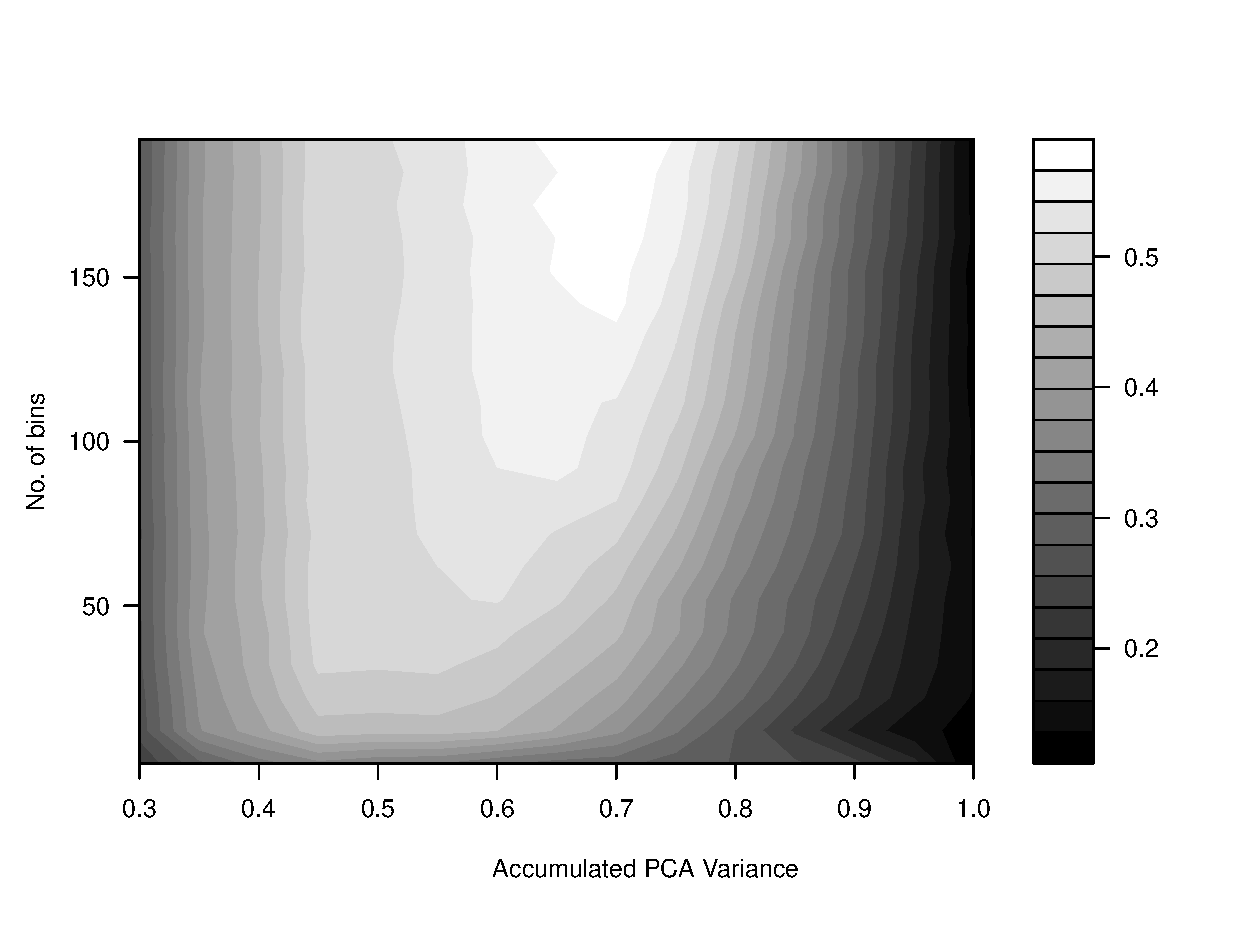
\includegraphics[width = \textwidth]{graphics/contour_bins_vs_pca}
\caption{Contour of the success rate of the Naive Bayes with accumulated PCA going from 0.3 to 1 and the number of bins from 2 to 192.
The data was normalized using z-score first and the Laplace value was set to 1.
The contour was created with G3M2's data in the test set and the remaining 15 loadable datasets in the training set.}
\label{fig:contour_bin-vs-pca}
\end{figure}

From figure \ref{fig:contour_bin-vs-pca} it can be seen that the best point goes out of the view, and is in fact increasing, indicating that it gets better the higher dimensional the data is. The best bin size can hence not be determined. The most optimum point would be around 40 bins and an accumulative PCA of 50\% as at this point, the increase PCA and bins does not improve the success by an considerably enough compared to how much the timing would increase.

The Laplace value of the Naive Bayes was also tested, but due to unknown reasons, then the Laplace coefficient did not have any effect on the success of the method.
It was therefore decided not to show the effect of such in this report.

\subsubsection{Pixel Bin Occurrence}
A contour of the number of bins used to represent a pixel and the number of horizontal stripes the image is divided into is shown in figure \ref{fig:contour_bin-vs-div}.

\begin{figure}[H]
\centering
%\includegraphics[width = \textwidth]{graphics/contour_bins_vs_div}
\caption{Contour of the success rate of the Naive Bayes with the number of bins used to represent a pixel and the number of horizontal stripes the image is divided into.
The contour was created with G3M2's data in the test set and the remaining 15 loadable datasets in the training set.}
\label{fig:contour_bin-vs-div}
\end{figure}

It can be seen on figure \ref{fig:contour_bin-vs-div} that ... graph to be seen...



\subsubsection{Selection of the Methods}
Comparing the two graphs in figure \ref{fig:contour_bin-vs-pca} and \ref{fig:contour_bin-vs-div} it can clearly be seen that the first method used for figure \ref{fig:contour_bin-vs-pca} performs considerably better than the other method proposed.
It was therefore decided only to continue with the better method.
